\documentclass{article}
\usepackage[utf8]{inputenc}
\usepackage{amsmath}
\usepackage{physics}
\usepackage{dsfont}
\usepackage{graphicx}
\usepackage{listings}
\usepackage{color}

% ---------------------------------------------------------------
\title{CSE 546: Homework 0}
\author{Andy Goldschmidt}
\date{Due: 10/4/18}
% ---------------------------------------------------------------
\begin{document}

\maketitle

\section{Analysis}

\paragraph{1.1}\ \newline
(a) Consider $x,y \in S := \{ x \in \mathds{R}^n: \norm{x} \le 1 \} $ and $\lambda \in [0,1]$. Compute:
\begin{align}
    \norm{\lambda x + (1-\lambda) y}
    &\le \norm{\lambda x} + \norm{(1-\lambda) y} \label{te} \\
    &=  \abs{\lambda} \norm{x} + \abs{1 - \lambda} \norm{y} \label{as} \\
    &=  \lambda \norm{x} + (1 - \lambda) \norm{y} \\
    &\le  \lambda + (1 - \lambda) \label{setdef} \\
    &= 1
\end{align}
Line \ref{te} uses triangle inequality, line \ref{as} uses absolutely scalability, and line \ref{setdef} uses the definition of S.
\newline
\newline 
(b) We will proceed by counterexample to show $\norm{x} := (\sum _{i=1}^{n}{\abs{x_i}^{1/2}})^2$ is not a norm. Consider x=(0,1) and y=(1,0). Compute:
\begin{align}
    \norm{x+y} 
    &= \norm{(1,1)} \\
    &= (1^{1/2}+1^{1/2})^2 \\
    &= 4
\end{align}
while
\begin{align}
    \norm{x}+\norm{y} 
    &= \norm{(0,1)} + \norm{(1,0)} \\
    &= (0^{1/2}+1^{1/2})^2 + (1^{1/2}+0^{1/2})^2 \\
    &= 2
\end{align}
so that $\norm{x+y} > \norm{x}+\norm{y}$, contradicting the triangle inequality.

\paragraph{1.2}\ Show: $\norm{x}_\infty \le \norm{x}_2 \le \norm{x}_1$. \newline
For the first inequality (w.l.o.g. let $\norm{x}_\infty=\abs{x_1}$):
\begin{align}
    \norm{x}_\infty
    &=(x_1^2)^{1/2} \\
    &\le ({x_1}^2 + \sum_{i=2}^{n}{x_i}^2)^{1/2} \\
    &= \norm{x}_2
\end{align}
For the second inequality:
\begin{align}
    \norm{x}_2 
    &=(\sum _{i=1}^{n}{\abs{x_i}^{2}})^{1/2} \\
    &\le (\sum _{i=1}^{n}{\abs{x_i}^{2}} + \sum _{i\ne j}{\abs{x_i}\abs{x_j}})^{1/2} \label{crossterms} \\
    &=((\sum _{i=1}^{n}{\abs{x_i}})^2)^{1/2} \label{factor1} \\
    &= \norm{x}_1
\end{align}
where we add in the positive-valued cross terms in line \ref{crossterms} and factor in line \ref{factor1}.

\paragraph{1.3}\ \newline
Let $A,B \in \mathds{R}^{n \cross n}$ have entries labeled $(a_{ij}), (b_{ij})$. Let $c \in \mathds{R}$. Define $f(x,y)=x^T A x + y^T B x + c$. Compute: $\grad_x$ and $\grad_y$. We will do this by rewriting f where repeated indices mean implied sums.
\begin{equation}
    f(x,y) = x_j a_{ji} x_i + y_j b_{ji} x_i + c
\end{equation}
Now compute:
\begin{align}
    \grad_x f(x,y) 
    &= \partial_{x_k}( x_j a_{ji} x_i  + y_j b_{ji} x_i + c ) \hat{k} \\
    &= (\partial_{x_k}( x_j ) a_{ji} x_i + x_j a_{ji} \partial_{x_k}(x_i) + y_j b_{ji} \partial_{x_k}(x_i)) \hat{k} \\
    &= (\delta_{kj} a_{ji} x_i + x_j a_{ji} \delta_{ki} + y_j b_{ji} \delta_{ki}) \hat{k} \\
    &= (a_{ki} x_i + x_j a_{jk} + y_j b_{jk}) \hat{k} \\
    &= A x + A^T x + B^T y
\end{align}
Similarly:
\begin{align}
    \grad_y f(x,y) 
    &= \partial_{y_k}( x_j a_{ji} x_i  + y_j b_{ji} x_i + c ) \hat{k} \\
    &= (\partial_{y_k}(y_j) b_{ji} (x_i)) \hat{k} \\
    &= (\delta_{kj} b_{ji} (x_i)) \hat{k} \\
    &= (b_{ki} (x_i)) \hat{k} \\
    &= B x
\end{align}

\paragraph{1.4}\ \newline
Every matrix in this problem shares the same set of eigenvectors. Suppose A and B have eigenvalues $a_i$ and $b_i$, respectively. The desired eigenvalues are:
\begin{align*}
(a)&\ C = A + B: a_i + b_i \\
(b)&\ D = A - B: a_i - b_i \\
(c)&\ E = AB: a_i*b_i \\
(d)&\ F = A^{-1}B:  b_i/a_i
\end{align*}
The quickest way to see this is to express the two operators A and B as diagonal matrices in their shared eigenbasis. After rewriting, the matrix operations remaining are straightforward and immediately yield the eigenvalues of these newly computed matrices. (For part (d), the inverse matrix is unique so the form of $A^{-1}$ can be checked).

\paragraph{1.5}\ \newline
(a) Given $x,y \in \mathds{R}^n$, compute: 
\begin{equation}
  x^T (y y^T) x = ( x^T y ) ( y^T x ) = (y^T x)^T (y^T x) = (y^T x)^2 \ge 0
\end{equation}
We have been somewhat loose here in justifying the exchange of parenthesis that lets the matrix $y y^T$ split to act separately on both x and $x^T$ in their spaces. We could show this by playing with indices, but it's possibly quicker to see in the following notation: $x^T (yy^T) x \longrightarrow \bra{x}(\ket{y}\bra{y})\ket{x} = \bra{x}\ket{y}\bra{y}\ket{x} $. What remains in the last result is simply a constant squared.
\newline 
\newline
(b) Let $X \in \mathds{R}^n$ be a random vector. $\forall y \in \mathds{R}^n$, compute:
\begin{align}
    y^T \Sigma y 
    &= y^T \mathds{E}[(X-\mathds{E}[X])(X-\mathds{E}[X])^T] y \\
    &= \mathds{E} [y^T (X-\mathds{E}[X])(X-\mathds{E}[X])^T y ] \label{linofexp} \ge 0
\end{align} 
In line \ref{linofexp}, we use the linearity of expectation and note that from part (a) the quantity in the expectation is positive. The expectation of a positive quantity is positive so we have shown that $\Sigma$ is postive semi-definite.
% \newline
% \newline
(c) Suppose A is a symmetric matrix so that $A=U\text{diag}(\alpha)U^T$ with $U^TU=I$. We want to show that A is positive semi-definite $\Leftrightarrow \underset{i}{\text{min }}\alpha_i \ge 0$.
\newline
($\Leftarrow$) Suppose the latter, and consider the basis where A is diagonal. Note that an inner product is independent of basis so we can prove our positive semi-defininte result in any basis. $\forall x$ in this basis we have:
\begin{equation}
    x^T A x = \sum_{i=1}^{n} x_i \alpha_i x_i = \sum_{i=1}^{n} {x_i}^2 \alpha_i \ge 0
\end{equation}
where we use the assumption to assert the final inequality.
\newline
($\Rightarrow$) Now suppose A is positive semi-definite and that $\underset{i}{\text{min }}\alpha_i < 0$. W.l.o.g. let this minimal index be 1. Now $\exists x$ such that
\begin{equation}
    x^T A x = x_1 \alpha_1 x_1 = {x_1}^2 \alpha_1 < 0
\end{equation}
This contradicts the assumption that A was positive semi-defininte.

\paragraph{1.6}\ \newline
(a) Let X and Y be random variables with PDFs f and g, respectively. Consider Z=X+Y. We will throw caution to the wind and use a continuous version of the law of total probability:
\begin{align}
    P(Z=z)
    &=P(X+Y=z) \\
    &=\int \dd{x} P(X+Y=z | X=x) P(X=x) \\
    &=\int \dd{x} P(Y=z-x) P(X=x) \\
    &=\int \dd{x} g(z-x) f(x) =: h(z)
\end{align}
\newline
\newline
(b) Suppose X and Y are both independent and uniformly distributed on [0,1]. Compute:
\begin{align}
    h(z)
    &=\int_0^1 \dd{x} f(x) g(z-x) \\
    &=\int_0^1 \dd{x} g(z-x) \\
    &=\int_{z-1}^{z} \dd{u} g(u) \\
    &=
    \begin{cases}
        \int_{0}^{z}\dd{u} = z, z \le 1 \\
        \int_{z-1}^{1}\dd{u} = 2-z, z \ge 1
    \end{cases} \\
    &= 1-\abs{z-1}
\end{align}
\newline
\newline
(c) Compute:
\begin{align}
    P(X \le 1/2 | X+Y \ge 5/4) 
    &= \frac{P(X \le 1/2 \cap X+Y \ge 5/4)}{P(X+Y \ge 5/4)} \\
    &= \frac{(1/2)(1/4)^2}{(1/2)(3/4)^2} = \frac{1}{9}
\end{align}
The most effective argument comes from geometry and would be aided by pictures that are not included here.

\paragraph{1.7}\ \newline
We want the adjusted random variable: $(X-\mu)/\sigma$. With this choice we have
\begin{align}
    E[(X-\mu)/\sigma]
    &=E[(X-\mu)/\sigma] \\
    &=(E[X]-\mu)/\sigma = 0
\end{align}
and
\begin{align}
    &E[((X-\mu)/\sigma-E[(X-\mu)/\sigma])^2] \\
    &=E[((X-\mu)/\sigma - 0)^2]\\
    &=E[(X-E[X])^2]/\sigma^2 = 1
\end{align}
as desired.

\paragraph{1.8}\ \newline
(a) $\forall x$, compute:
\begin{align}
    E[\hat{F}_n(x)]
    &=E[\frac{1}{n}\sum_{i=1}^{n}I\{X_i \le x\}]\\
    &=\frac{1}{n}\sum_{i=1}^{n}E[I\{X_i \le x\}]\\
    &=\frac{1}{n}\sum_{i=1}^{n}F(x)=F(x)
\end{align}
\newline
\newline
(b) $\forall x$, compute:
\begin{align}
    E&[(\hat{F}_n(x)-F(x))^2] \\
    &=E[{\hat{F}_n(x)}^2]-F(x)^2 \\
    &=E[(\frac{1}{n}\sum_{i=1}^{n}I\{X_i \le x\})^2]-F(x)^2 \\
    &=\frac{1}{n^2} E[\sum_{i=1}^{n}I\{X_i \le x\} + \sum_{i\ne j}I\{X_i \le x\}I\{X_j \le x\}]-F(x)^2 \label{indicator} \\
    &=\frac{1}{n} E[I\{X_1 \le x\}] + \frac{n(n-1)}{n^2} E[I\{X_1 \le x\}I\{X_2 \le x\}]-F(x)^2 \label{counting} \\
    &=\frac{1}{n} F(x) + \frac{n-1}{n} F(x)^2 - F(x)^2 \\
    &=\frac{1}{n} F(x)(1-F(x))
\end{align}
We arrive at Eq. \ref{indicator} by noting the idempotency of an indicator function. For Eq. \ref{counting}, we use that each random variable is identically distributed and count the elements in each sum.
\newline
\newline
(c) Using part b., we can bound:
\begin{align}
    &\underset{x \in \mathds{R}}{\text{sup}} E[(\hat{F}_n(x)-F(x))^2] \\
    =&\underset{x \in \mathds{R}}{\text{sup}} \frac{1}{n} F(x)(1-F(x)) \\
    \le& \frac{1}{n}\frac{1}{2}(1-\frac{1}{2}) = \frac{1}{4n} \label{inequality}
\end{align}
We use some calculus to argue $y(1-y)$ is maximal at $y=1/2$.

\section{Programming}

\paragraph{2.9}
For (a) and (b), we are to produce Fig. \ref{fig:plot9}. We choose $n=40,000$ in the inequality in Eq. \ref{inequality} for the bound $\underset{x \in \mathds{R}}{\text{sup}} \sqrt{E[(\hat{F}_n(x)-F(x))^2]} \le 0.0025$ to hold. Fig. \ref{fig:plot9} shows that the sum of k independent, zero-mean random variables with variance 1/k converges to a standard-normal distribution as $k\longrightarrow\infty$. The figure shows this by plotting the empirical cumulative distribution functions of such sums of random variables and comparing these to the cumulative distribution function of a standard-normal-distributed random variable.

My code:
\lstinputlisting[language=Python, frame=Single, breaklines=true]{problem_9.py}

\begin{figure}
  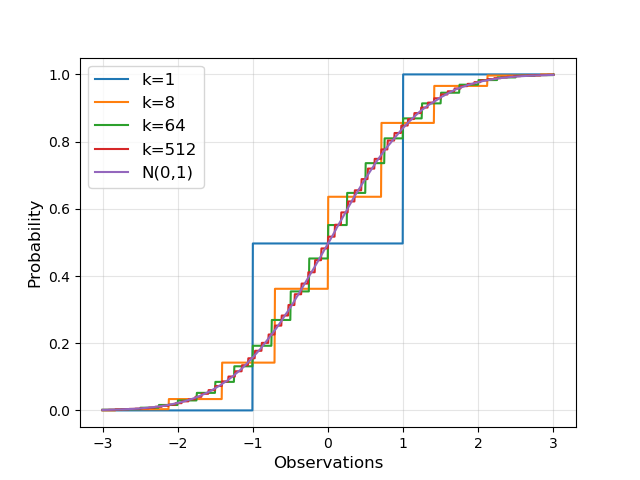
\includegraphics[width=\linewidth]{plot_hw0p9.png}
  \caption{The figure shows $\hat{F}_n(x)=\frac{1}{n} \sum_{j=1}^{n} I\{Y^{(k)}_j\le x\}$ where $Y^{(k)}_j=\frac{1}{\sqrt{k}}\sum_{i=1}^{k}{B_i}$ for n=40,000 for various values of k. For reference the plot includes $\hat{F}_n(x)=\frac{1}{n} \sum_{i=1}^{n} I\{Z_i\le x\}$ with standard-normal random variables $Z_i \sim N(0,1)$ because these will have exactly the empirical cumulative distribution function that the central limit theorems asserts $Y^{(k)}$ approaches in the large k limit.}
  \label{fig:plot9}
\end{figure}

\end{document}
% ---------------------------------------------------------------

